\documentclass[11pt]{article}

\usepackage[left=2cm, right=2cm, top=2cm]{geometry}
\usepackage[dvipdfmx]{graphicx}
\usepackage{float}
\usepackage{hyperref}

\hypersetup{
    colorlinks=true,
    linkcolor=black,
    filecolor=magenta,      
    urlcolor=blue,
}

\providecommand{\e}[1]{\ensuremath{\times 10^{#1}}}

\title{Project 1: Reaction Timer}
\author{Jacob Boline}

\begin{document}
\maketitle

\section{Introduction}
In this project I was tasked with creating and testing a design that would measure a humans response to visual stimulus. The device is required to have 3 buttons that correspond to start, stop, and clear. The basic premise of the design is to have a random delay of 2-15 seconds after the start button is pushed, but before the LED is lit. Once the LED is lit, a 4-digit display will show the number of milliseconds it takes a person to press the stop button. In addition, there are some extra features added to make the design more robust such as a state if the stop button is pushed too early, or not pushed at all. To accomplish this project Vivado 2017.2 was used to simulate, synthesize, and implement System Verilog code for a Basys 4 DDR development board. The project design files can be found at: \url{https://github.com/txjacob/SoC_FPGA}

\section{Experimental Plan}
For this design five fundamental Modules are needed:
\begin{enumerate}
    \item 7-seg Driver
    \item Random Number Generator
    \item Universal Counter
    \item Stopwatch
    \item State Machine
\end{enumerate}

\subsection{7-Seg Driver Module}

\begin{figure}[H]
	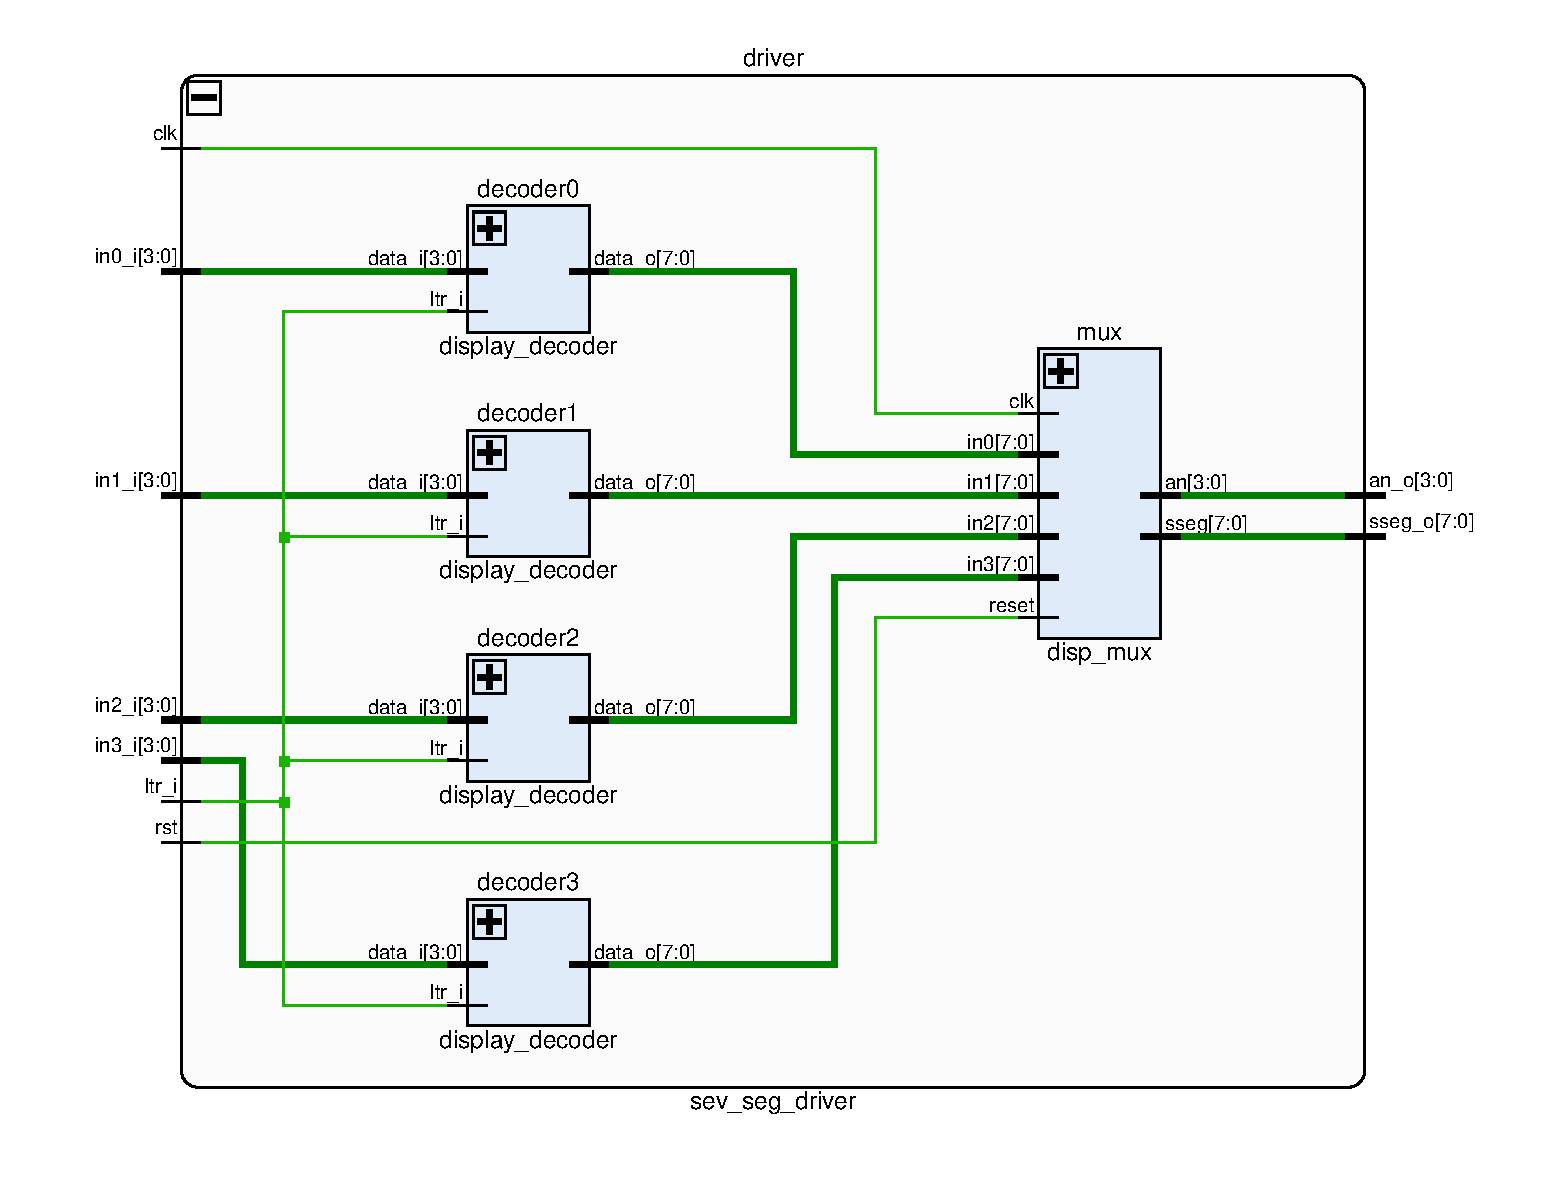
\includegraphics [width=5in]{display_driver.eps}
	\centering
	\caption{Block diagram of 7-seg driver module.}
	\label{fig:7SegDriver}
\end{figure}

The first step to building this design was to create a method for driving the 7-segment display. This was accomplished by creating a decoder that had a 4-bit data in port, a 1-bit flag to indicate whether the data corresponded to numerical values, or alphabetic values, and an 8-bit data out port that corresponds to what portions of 7-segment display to turn on. Using 4 instantiations of this decoder, and the display mux from listing 4.15 in the class textbook I created a driver module (as seen in Figure \ref{fig:7SegDriver}) that had 4 separately controlled digits, and could display the numbers 0-9 and the letters H and I.

\subsection{Random Number Generator Module}

\begin{figure}[H]
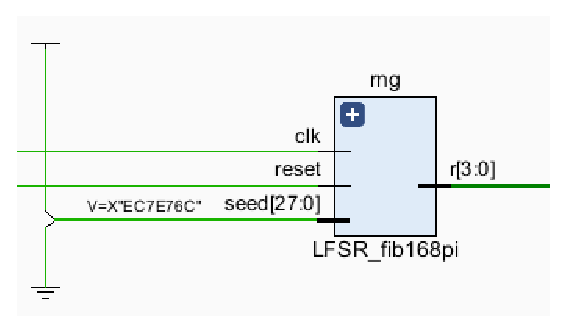
\includegraphics [width=4in]{lfsr.eps}
	\centering
	\caption{Block diagram of LFSR module.}
	\label{fig:LFSRmod}
\end{figure}

The random number generator module (Figure \ref{fig:LFSRmod}) is a modified version of the lfsr\_fib168pi design provided. In order to fit better into the project I modified the output to be a 4-bit number instead of a single bit. This was done by reading the first four bits of the state variable instead of using the straight polynomial variable. The 4-bits from the state variable were then passed through some combinational logic to limit the range of random numbers to be between 2 and 15. This was done by checking to see if the top 3-bits were all 1s, if they were then the two's place bit was zeroed out, if not the data was allowed to pass through. Finally, the data was summed with the number 2, and output from the module.

\subsection{Universal Counter Module}

\begin{figure}[H]
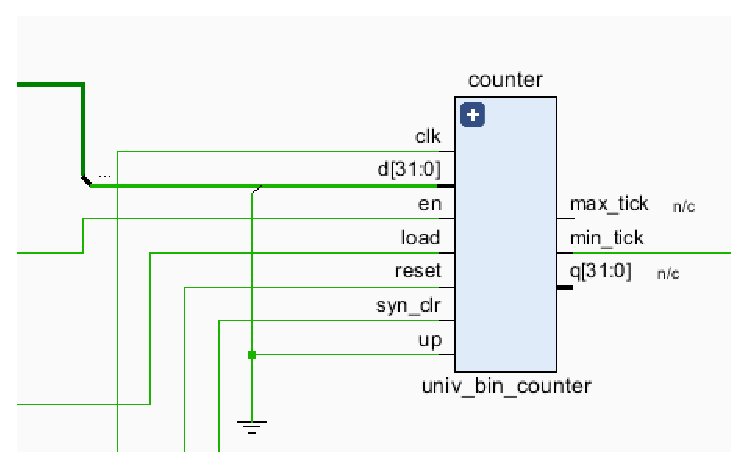
\includegraphics [width=4in]{counter.eps}
	\centering
	\caption{Block diagram of the Universal Counter module.}
	\label{fig:counterMod}
\end{figure}

The universal counter module (Figure \ref{fig:counterMod}) is taken from Listing 4.12. It was configured to be in countdown mode so that the state machine only has to wait for the zero flag to go high. The input of the counter was connected to the output of the random number generator multiplied by 100,000,000. This was done to convert the value in seconds to the number of 100 MHz clock cycles. Finally, three flags were created to control the counter: clear\_counter, load\_counter, and enable\_counter. Using these 3 flags the counter configuration can be individualized for each state.

\subsection{Stopwatch Module}

\begin{figure}[H]
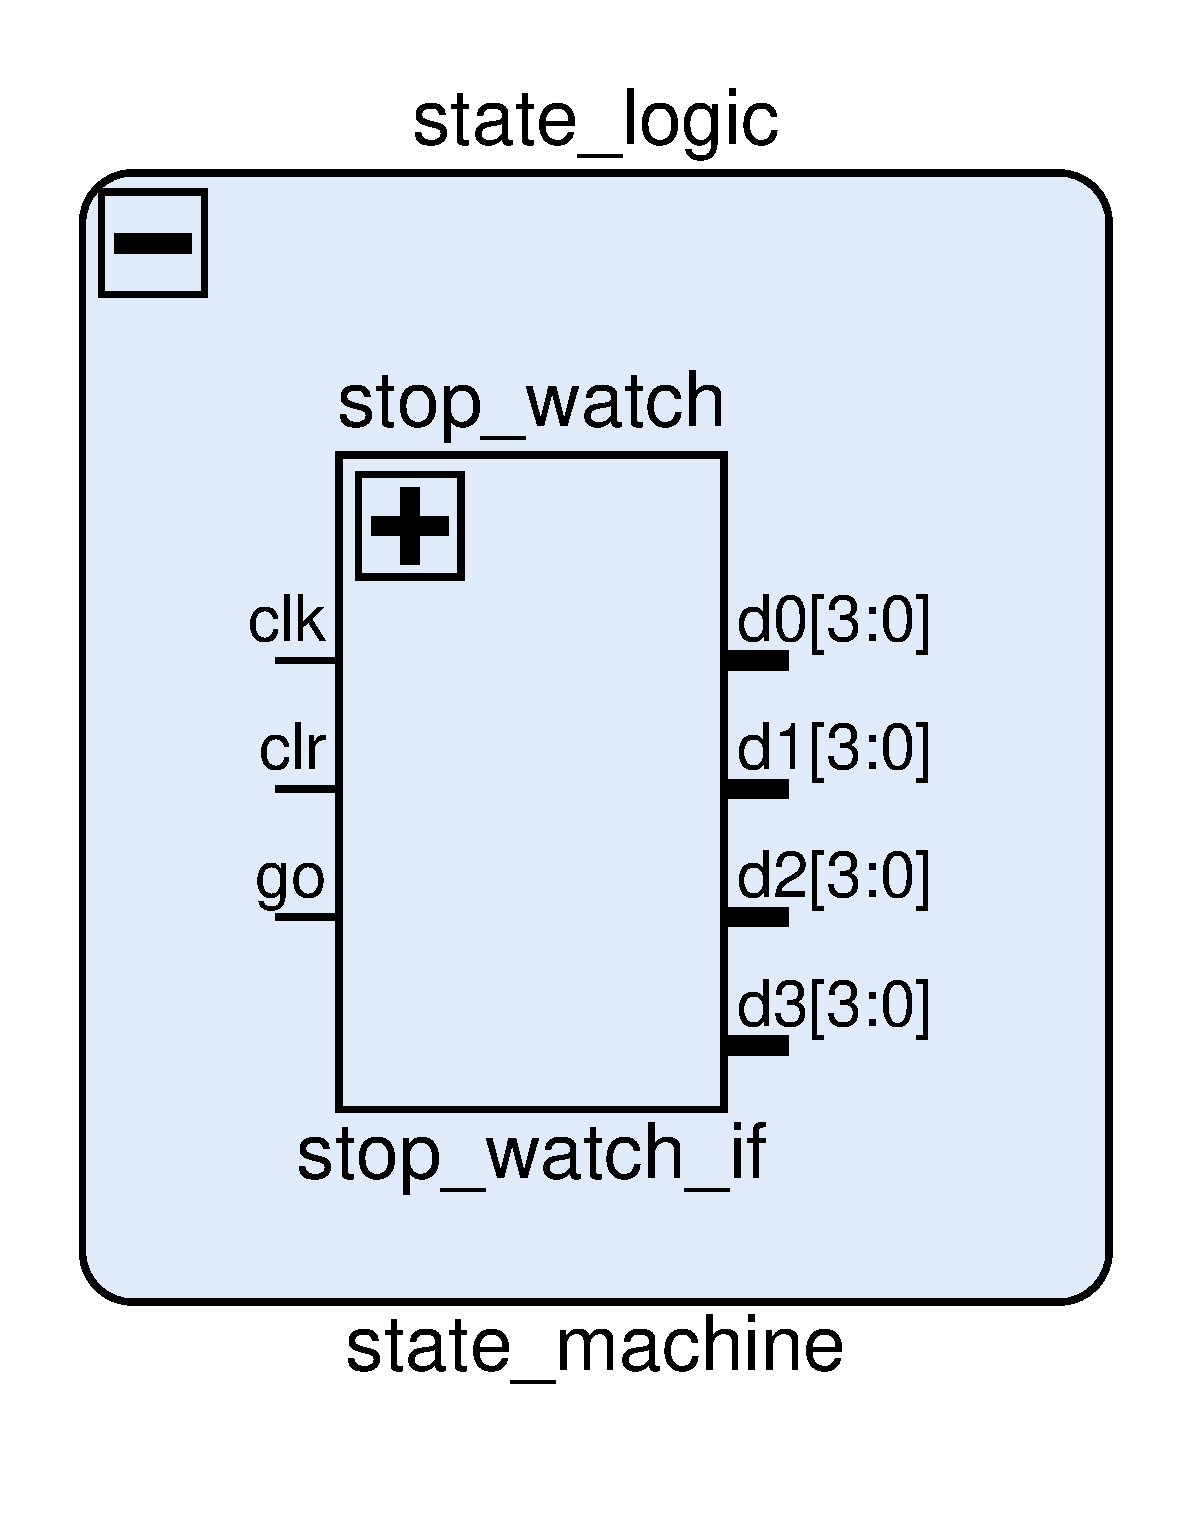
\includegraphics [width=2in]{stopwatch.eps}
	\centering
	\caption{Block diagram of the stopwatch module.}
	\label{fig:stopwatchmod}
\end{figure}

The stopwatch module (Figure \ref{fig:stopwatchmod}) is a modified version of the stop watch design in listing 4.20 of the class text book. To make the module more applicable for my design I extended the output to use all 4 digits on the 7-segment display, and adjusted the 1 ms tick generator factor. The factor was derived in the following manner:

\begin{center}
    $factor = \frac{100\e{6}\; cycles/s}{1\e{-3}\; ms/s} = 100\e{3}\; cycles/ms$
\end{center}
Using the clear and go pins of the module, the stopwatch can be started, stopped, and cleared independently in each state. In addition, the digit outputs are either connected to the the display driver, or left open depending on the current state.

\subsection{State Machine Module}
For the state machine I elected to use states that corresponded to six different states in the design's sequence. The six states are listed below and an ASMD diagram is shown in Figure \ref{fig:state_diagram}.

\begin{enumerate}
    \item init
    \item start
    \item delay
    \item count
    \item stop
    \item bad\_stop
\end{enumerate}


\subsubsection{init state}
The function of the init state is simple. While in this state "HI" is printed to the 7-segment, the stopwatch is cleared, and the universal counter is cleared. This state can only be reached either by pressing the global reset button, or from the stop and stop\_bad states. This state can only be exited by pressing the start button on the board, at which point the start state is entered.

\subsubsection{start state}
While in the start state the the display is blanked and the universal counter is loaded by asserting the load\_counter pin to HIGH. This state immediately transitions to the delay state on the next clock cycle.

\subsubsection{delay state}
In this state the load count pin is set to LOW, and the enable counter pin is set to HIGH. This allows the counter to latch in a random value and count down from that value. This state is exited once the universal counter hits zero (at which point the zero\_count flag will be asserted) or if the stop button is pushed. If the stop button is pushed the bad\_stop state will be entered, but if the button is never pushed before the universal counter reaches zero then the count state will be entered.

\subsection{count state}
Once the count state is entered the output of the stopwatch is connected to the 7-segment driver module, the LED is turned on, and the stop watch is started by asserting timer\_go to HIGH. This state is stayed in until the stop button is pushed, or the stopwatch reaches 1000ms, whichever comes first.

\subsubsection{stop state}
In this state the timer is stopped by asserting timer\_go to LOW. This causes the stopwatch to stop thus displaying the time it took for the stop button to be pressed after the LED was turned on. This state can only be exited by pressing the clear button, at which point the init state will be entered and the process will begin again.

\subsubsection{bad\_stop state}
This state is only entered if the stop button is pushed while in the delay state (and the universal counter has not yet reached zero). Once in this state the counter will be disabled, and "9999" will be displayed on the 7-segment. The only was to exit this state is by pressing the clear button, which will return the user to the init state.

\pagebreak
\begin{figure}[H]
	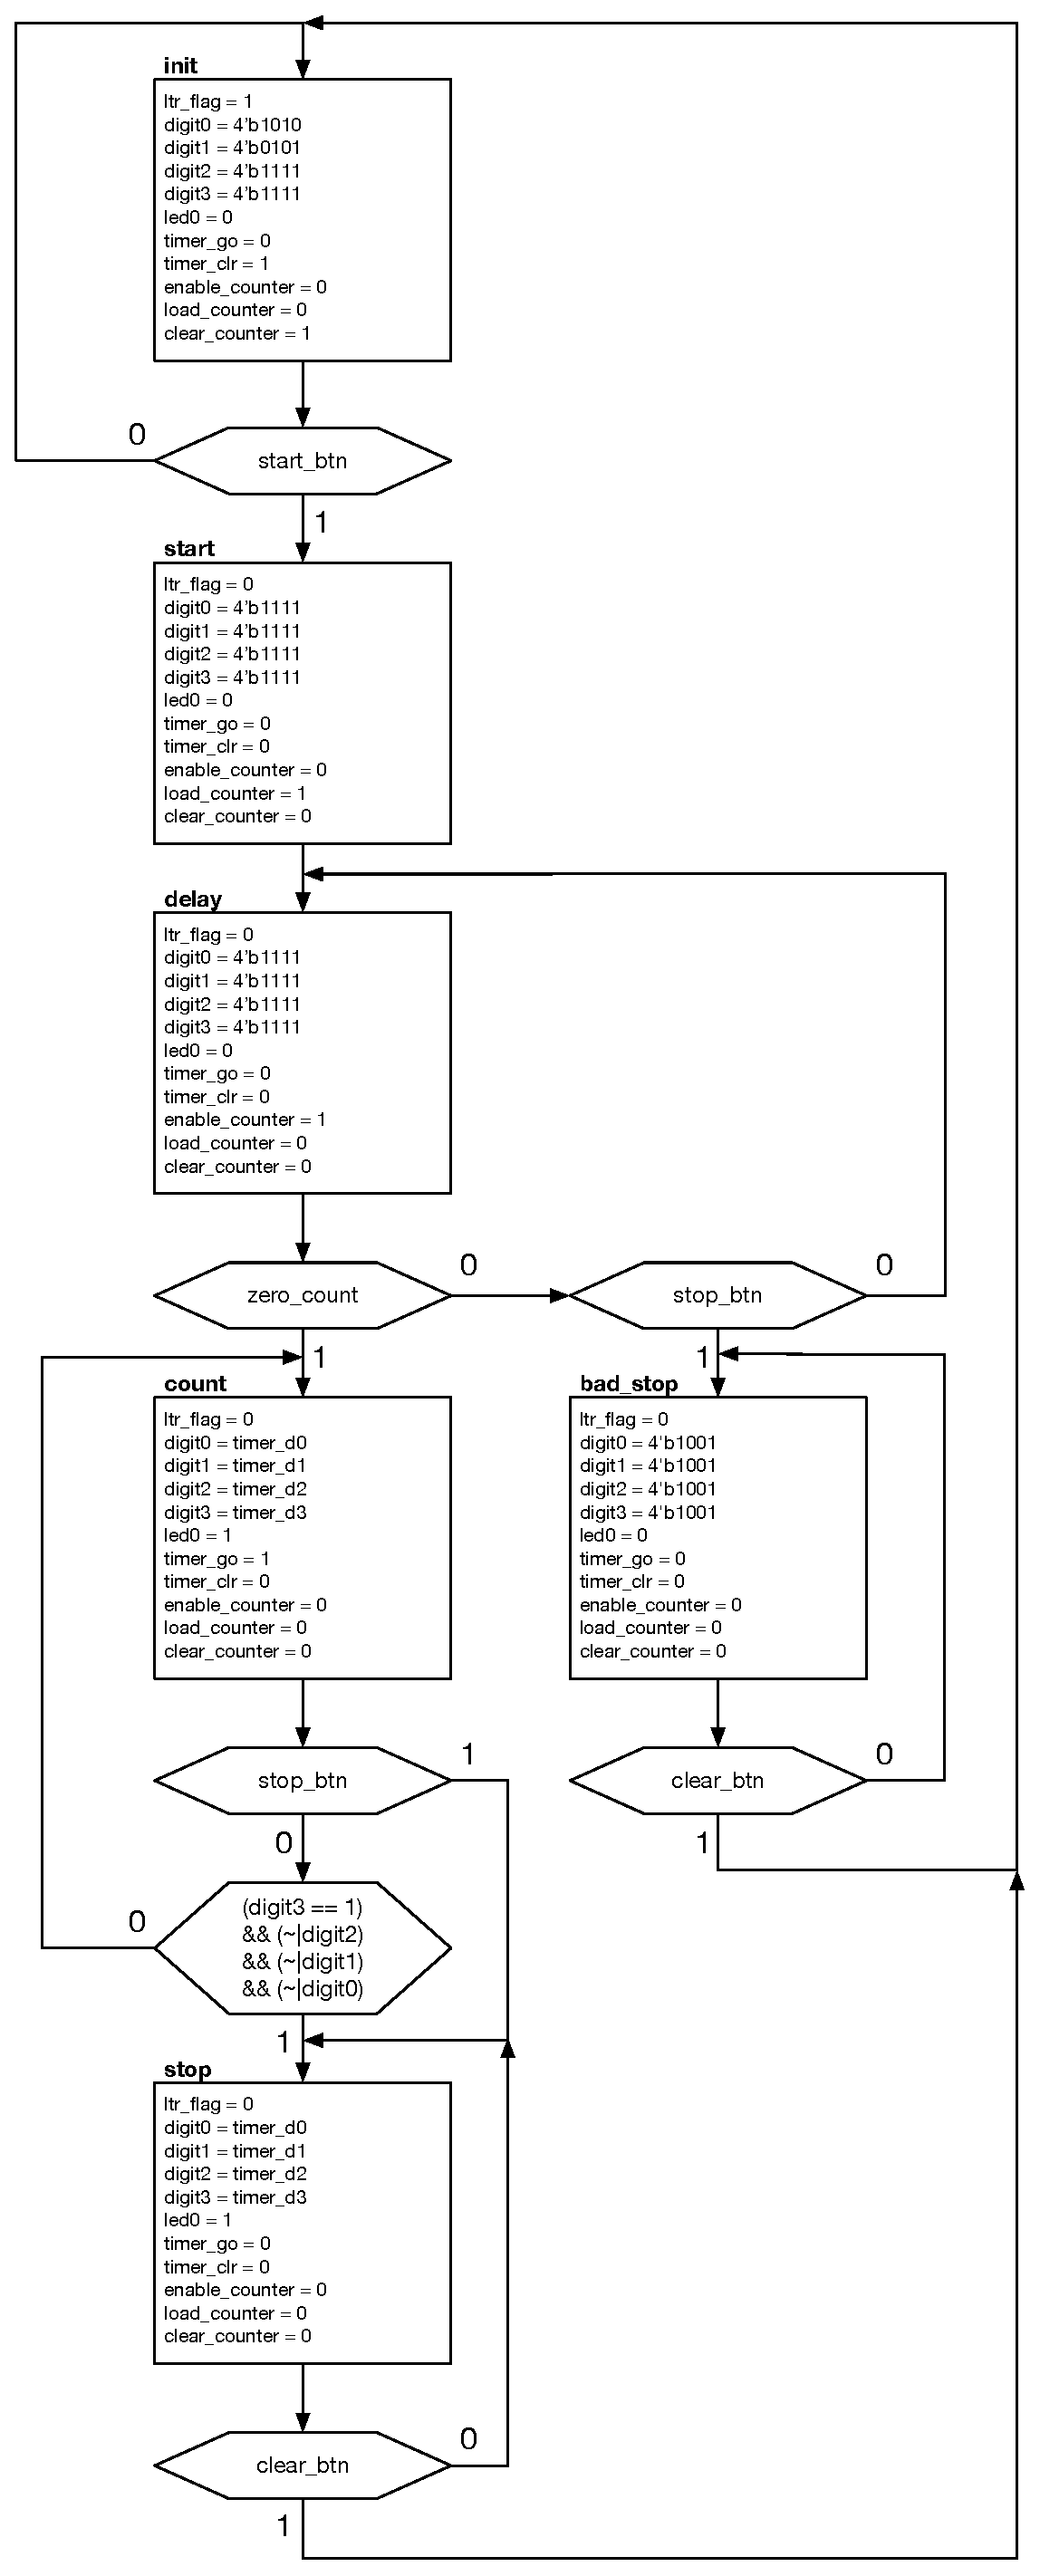
\includegraphics [width=3.45in]{state_diagram.eps}
	\centering
	\caption{State diagram of the reaction timer design}
	\label{fig:state_diagram}
\end{figure}

\section{Analysis}

\section{Conclusion}

\end{document}